% Figure from MATH 591 notes, Roadmap (front matter): the equations and quotients threads. Compile with the notes preamble.
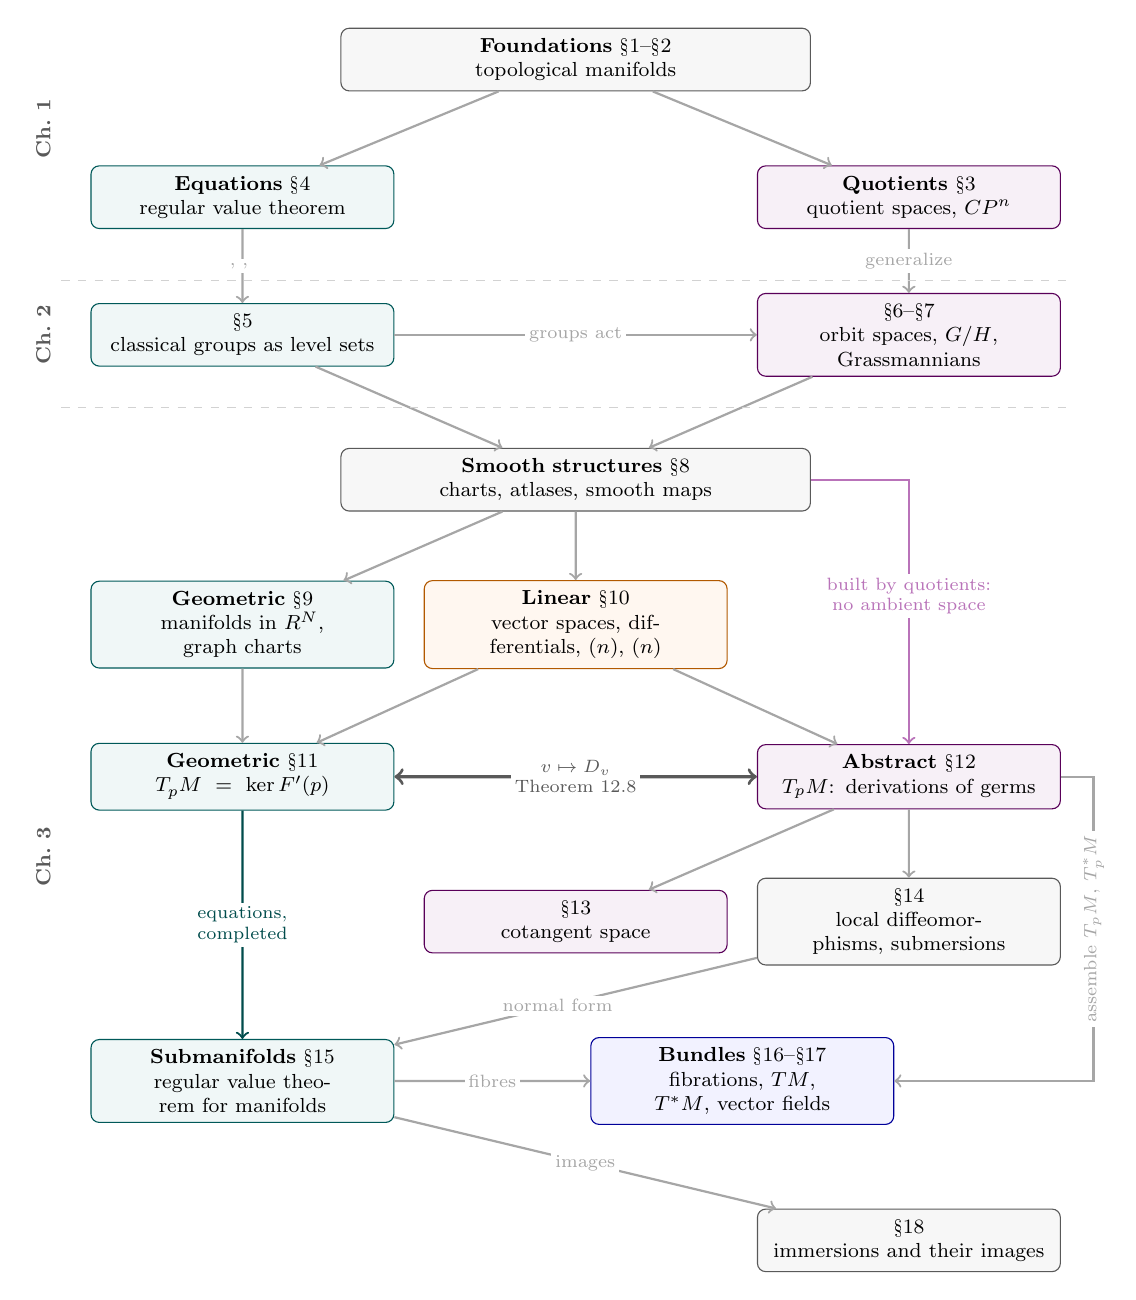
\begin{tikzpicture}[scale=0.92, transform shape]
\node[draw=gray!70!black, fill=gray!6, rounded corners=3pt, text width=6.2cm, align=center, font=\footnotesize, inner sep=4pt] (F) at (4.6,0) {\textbf{Foundations} \S1--\S2\\ topological manifolds};
\node[draw=teal!70!black, fill=teal!6, rounded corners=3pt, text width=3.9cm, align=center, font=\footnotesize, inner sep=4pt] (E1) at (0,-1.9) {\textbf{Equations} \S4\\ regular value theorem};
\node[draw=violet!70!black, fill=violet!6, rounded corners=3pt, text width=3.9cm, align=center, font=\footnotesize, inner sep=4pt] (Q1) at (9.2,-1.9) {\textbf{Quotients} \S3\\ quotient spaces, $\mathbb{CP}^n$};
\node[draw=teal!70!black, fill=teal!6, rounded corners=3pt, text width=3.9cm, align=center, font=\footnotesize, inner sep=4pt] (E2) at (0,-3.8) {\S5\\ classical groups as level sets};
\node[draw=violet!70!black, fill=violet!6, rounded corners=3pt, text width=3.9cm, align=center, font=\footnotesize, inner sep=4pt] (Q2) at (9.2,-3.8) {\S6--\S7\\ orbit spaces, $G/H$, Grassmannians};
\node[draw=gray!70!black, fill=gray!6, rounded corners=3pt, text width=6.2cm, align=center, font=\footnotesize, inner sep=4pt] (S) at (4.6,-5.8) {\textbf{Smooth structures} \S8\\ charts, atlases, smooth maps};
\node[draw=teal!70!black, fill=teal!6, rounded corners=3pt, text width=3.9cm, align=center, font=\footnotesize, inner sep=4pt] (G1) at (0,-7.8) {\textbf{Geometric} \S9\\ manifolds in $\mathbb{R}^N$, graph charts};
\node[draw=orange!70!black, fill=orange!6, rounded corners=3pt, text width=3.9cm, align=center, font=\footnotesize, inner sep=4pt] (L) at (4.6,-7.8) {\textbf{Linear} \S10\\ vector spaces, differentials, $\Ogp(n)$, $\Ugp(n)$};
\node[draw=teal!70!black, fill=teal!6, rounded corners=3pt, text width=3.9cm, align=center, font=\footnotesize, inner sep=4pt] (T1) at (0,-9.9) {\textbf{Geometric} \S11\\ $T^{\geo}_pM = \ker F'(p)$};
\node[draw=violet!70!black, fill=violet!6, rounded corners=3pt, text width=3.9cm, align=center, font=\footnotesize, inner sep=4pt] (T2) at (9.2,-9.9) {\textbf{Abstract} \S12\\ $T_pM$: derivations of germs};
\node[draw=violet!70!black, fill=violet!6, rounded corners=3pt, text width=3.9cm, align=center, font=\footnotesize, inner sep=4pt] (C) at (4.6,-11.9) {\S13\\ cotangent space};
\node[draw=gray!70!black, fill=gray!6, rounded corners=3pt, text width=3.9cm, align=center, font=\footnotesize, inner sep=4pt] (M) at (9.2,-11.9) {\S14\\ local diffeomorphisms, submersions};
\draw[->, thick, gray!70] (F) -- (E1);
\draw[->, thick, gray!70] (F) -- (Q1);
\draw[->, thick, gray!70] (E1) -- node[font=\scriptsize, fill=white, inner sep=1.5pt] {$\SL$, $\Ogp$, $\Ugp$} (E2);
\draw[->, thick, gray!70] (Q1) -- node[font=\scriptsize, fill=white, inner sep=1.5pt] {generalize} (Q2);
\draw[->, thick, gray!70] (E2) -- node[font=\scriptsize, fill=white, inner sep=1.5pt] {groups act} (Q2);
\draw[->, thick, gray!70] (E2) -- (S);
\draw[->, thick, gray!70] (Q2) -- (S);
\draw[->, thick, gray!70] (S) -- (G1);
\draw[->, thick, gray!70] (S) -- (L);
\draw[->, thick, violet!55] (S.east) -| node[pos=0.72, font=\scriptsize, fill=white, inner sep=1.5pt, align=center] {built by quotients:\\ no ambient space} (T2.north);
\draw[->, thick, gray!70] (G1) -- (T1);
\draw[->, thick, gray!70] (L) -- (T1);
\draw[->, thick, gray!70] (L) -- (T2);
\draw[<->, very thick, black!65] (T1) -- node[font=\scriptsize, fill=white, inner sep=1.5pt, align=center] {$v \mapsto D_v$\\ Theorem~12.8} (T2);
\draw[->, thick, gray!70] (T2) -- (C);
\draw[->, thick, gray!70] (T2) -- (M);
\node[font=\footnotesize\bfseries, gray!70!black, rotate=90] at (-2.75,-0.95) {Ch.~1};
\node[font=\footnotesize\bfseries, gray!70!black, rotate=90] at (-2.75,-3.8) {Ch.~2};
\node[draw=teal!70!black, fill=teal!6, rounded corners=3pt, text width=3.9cm, align=center, font=\footnotesize, inner sep=4pt] (SM) at (0,-14.1) {\textbf{Submanifolds} \S15\\ regular value theorem for manifolds};
\node[draw=blue!60!black, fill=blue!5, rounded corners=3pt, text width=3.9cm, align=center, font=\footnotesize, inner sep=4pt] (BU) at (6.9,-14.1) {\textbf{Bundles} \S16--\S17\\ fibrations, $TM$, $T^*M$, vector fields};
\draw[->, thick, teal!60!black] (T1) -- node[font=\scriptsize, fill=white, inner sep=1.5pt, align=center] {equations,\\ completed} (SM);
\draw[->, thick, gray!70] (M) -- node[pos=0.55, font=\scriptsize, fill=white, inner sep=1.5pt] {normal form} (SM);
\draw[->, thick, gray!70] (SM) -- node[font=\scriptsize, fill=white, inner sep=1.5pt] {fibres} (BU);
\draw[->, thick, gray!70] (T2.east) -- ++(0.45,0) |- node[pos=0.25, font=\scriptsize, fill=white, inner sep=1.5pt, rotate=90] {assemble $T_pM$, $T_p^*M$} (BU.east);
\node[draw=gray!70!black, fill=gray!6, rounded corners=3pt, text width=3.9cm, align=center, font=\footnotesize, inner sep=4pt] (IM) at (9.2,-16.3) {\S18\\ immersions and their images};
\draw[->, thick, gray!70] (SM) -- node[pos=0.5, font=\scriptsize, fill=white, inner sep=1.5pt] {images} (IM);
\node[font=\footnotesize\bfseries, gray!70!black, rotate=90] at (-2.75,-11.0) {Ch.~3};
\draw[gray!35, dashed] (-2.5,-3.05) -- (11.4,-3.05);
\draw[gray!35, dashed] (-2.5,-4.8) -- (11.4,-4.8);
\end{tikzpicture}
